\section*{Introduction}
\addtocontents{toc}{\protect\setcounter{tocdepth}{0}}
Time series prediction (and related regressional tasks) is a subject of high interest across many disciplines of science and mathematics. The history of time series can be traced back to the birth of science in ancient Greece where Aristotle devised a systematic approach to weather forecasting in 350 BC in his famous treatise {\it Meteorologica}. This method was later used to help predict when certain meteorological induced events, such as the flooding of the Nile river \cite{10.2307/26254645}. Statistical modelling for time series prediction would not come until the $20^{\text{th}}$ century where development of AutoRegressive Moving Average (ARMA) models which where first mentioned by Yule \cite{YuleG.Udny1927OaMo} in 1927 and later popularized by Box and Jenkins in their book {\it Time Series Analysis} published in 1970 \cite{BoxGeorgeE.P.2008Tsa:}.

Given a data set of $n$ observations $\calD = \left\{ \left( x_i , y_i \right) \right\}_{i=1}^{n}$, where each input $x_i \in \RR_{>0}$ is a time value and $y_i \in \RR$ is a output or experimental observation that acts a function of time, the goal of time series prediction is to try and best predict a value $y_{\star}$ at time $x_{\star}$. With computing power becoming ever more advanced and affordable, many have taken to Machine Learning (ML) to develop sophisticated models to address the problem of creating accurate yet computationally inexpensive time series predictors. Broadly speaking, ML is any class of heuristic algorithm that attempts to refine and develope some model to perform a "simple" task by learning through user provided input. ML is founded on the idea that any form of task learning is done through sensory input taken from the surrounding environment. More formally speaking, ML attempts to generate a function $f : X \to Y$, for some input set $X$ and observation or output set $Y$, were the outputs given by $f$ closely aligns to actual observations. It is tacitly assumed  that the phenomena we are studying follows laws which admit mathematical formulation and that experimental results can be reproduced to some degree of accuracy. Typically, experiments will never produce exact values of the underpinning law, $g$. Instead experimental observations, $y_i$, will include a small amount of random error so that $y_i =  g(x_i) + \varepsilon_i$ where $\varepsilon_i \overset{\text{iid}}{\sim} \calN \left( 0, \sigma^2 \right)$.

A ML model will attempt to make accurate predictions using some simplified formulation of the world. The distribution corresponding to the probability of a prediction within the context of the "state of the world" is referred to as the {\it likelihood}. The uncertainty within the likelihood stems from the predictive limits of the model. These limitation usually arise as a consequence of selecting a model which is either too simple or complex. The "state of the world" is sometimes internally captured by the model as a set of mutable parameters $\bm{\theta}$. The process of taking observations and using them to form predictions is called {\it inference} which, in some sense, is synonymous with learning \cite{van2019sparse}.

ML can be applied to time series prediction in a fairly straight forward manner by simply teaching a ML algorithm the time series data set, $\calD$, to hopefully produce a function $f$ that serves as a good approximant for event prediction.

In this thesis we shall focus on a particular class of ML algorithms called Baysian models which, unsurprisingly, makes use of Bayesian statistics to drive inference. In Baysian models a {\it prior} distribution is used to quantify the uncertainty of the current state of the model before any observations are made. The model can then be updated once data is observed by using the likelihood to give a {\it posterior} distribution which represents the reduced uncertainty after "teaching" the model new observations. Methods of teaching a model how to change its behavior using a new set of observations often involves the use of a {\it loss function} $L$. The loss function is used as an aid in deciding what action, $a$, should be taken in to best minimize uncertainty. The best action, roughly speaking, can be evaluated as
\begin{equation*}
    a_{\text{opt}} =  \argmin_{a} \int L \left( y_{\star} , a \right) p \left( y_{\star} \mid \bm{x}_{\star}, \bm{X}, \bm{y} \right) \; d y_{\star}.
\end{equation*}
Interestingly, the best action does not rely so much on the model's internalized parameters but rather on the predictive distribution $p \left( y_{\star} \mid \bm{x}_{\star}, \bm{X}, \bm{y} \right)$ \cite{van2019sparse}. This key insight has spawned a class of ML algorithms that focuses on infering the function $f$ directly by computing $p \left( f \mid \calD \right)$ instead of finding optimal internal parameters using $p \left( \bm{\theta} \mid \calD \right)$ \cite{MurphyKevinP2012Ml}. Models that perform inference in this manner are called {\it non-parameteric} models. Within the {\it non-parameteric} model paradigm, the predictive distribution can be represented as
\begin{equation*}
    p \left( y_{\star} \mid x_{\star} , \bm{X} , \bm{y} \right) = \int p \left( y_{\star} \mid f , x_{\star} \right) p \left( f \mid \bm{X} , \bm{y} \right) \; df
\end{equation*}
and once new data is observed the posterior can be updated using Baye's rule
\begin{equation*}
    \text{posterior} = \frac{\text{likelihood} \times \text{prior}}{\text{marginal likelihood}}, \qquad p \left( \bm{f} , f_{\star} \mid \bm{y} \right) = \frac{p \left( \bm{y} \mid \bm{f} \right) p \left( \bm{f} , f_{\star} \right) }{p \left( \bm{y} \right)}
\end{equation*}
\cite{RasmussenCarlEdward2006Gpfm}. This thesis will focus on a particular non-parameteric Bayesian ML model called Gaussian processes (GPs). The over arching idea of GPs is to assign a prior probability to every possible function mapping from $X$ to $Y$. While this does not appear to be computationally tractable as this would due to the seemingly uncountable infinite number of mappings that would require checking, it turns out, these computations can infact be carried out given we are only seeking predictions at a finite number of points using a finite number of observations. GPs occupy a special place within the realm of ML since they account for uncertainty in a principled way, are relatively simple to implement and are highly modular allowing them to easily be incorporated into a larger systems. It is no surprise then that while other kernel methods (such as kernelized $k^{th}$ nearest neighbors and ridge regression) are still overshadowed by their neural network cousins, GPs have made a quiet comeback in the ML community \cite{cao2018scaling}.

The following example highlights a particular GP success story: a team of researchers led by Andries Potgieter at QAAFI (UQ) are currently investigating new digital approaches to accurately derive crop phenology stages (i.e. mid green, peak, flowering, grain filling and harvest) measured at field scale across large regions. Such methods can be used to better inform farmers and industry on the optimised time to plant various crops to minimize crop loss from environmental stresses such as frost and fungal disease. This involves analysing crop growth from previous seasons (i.e. 2018-2021) to forecast when certain phenological stages will take place in the current harvest. Outputs form this tool will allow producers to accurately map the temporal and spatial extend of phenology at a field and farm levels across different regions and seasons. This problem is readily converted into a time series problem. Originally, Potgieter's team surveyed a number of different parameteric models to carry out forecasting. However, the parameteric models we serverely limited in their ability to inform when key phenological stages would take place. After seeing the success of applying GPs to other remote senesing tasks \cite{rs14010146} investigated the use of GPs in their own research to find that they could produce much higher resolution predictions from which they could infer a far richer phenological timeline \cite{potg2013}. A comparision of using GPs over other parameteric models is shown in Figure \ref{fig: GP_motivate_wheat}.
\begin{figure}[h]
    \centering
    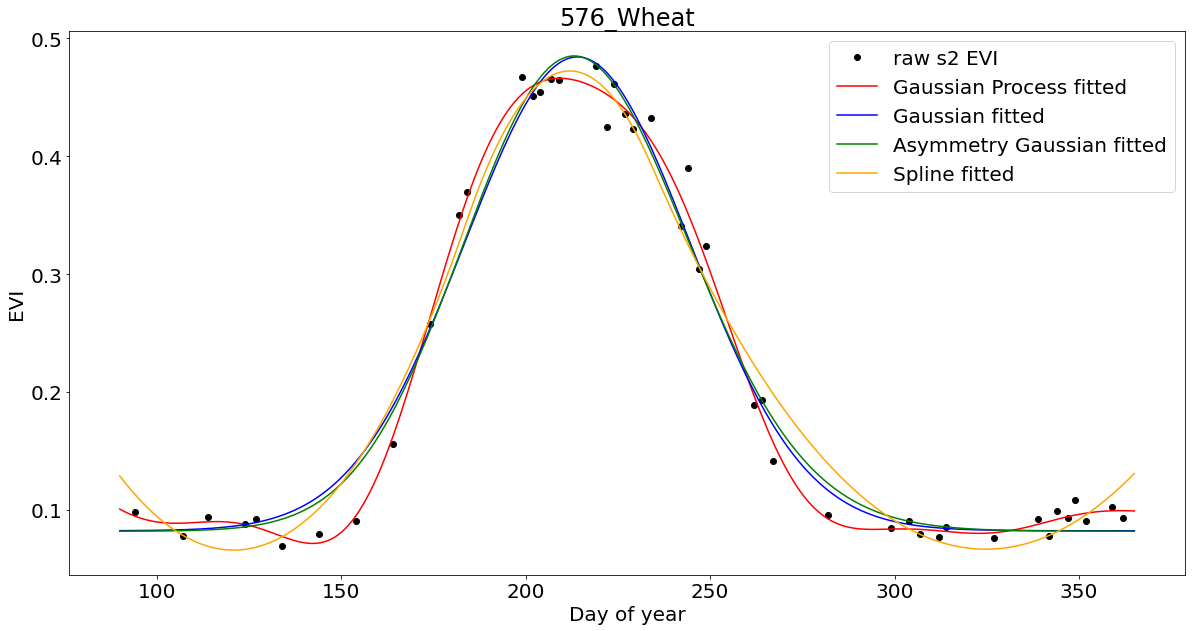
\includegraphics[scale=0.3]{img/yan_wheat_GPR_plot.png}
    \caption{Potgieter's team found that GPs where superior in terms of predicting a phenological timeline for a number of common seasonal crops over other parameteric models.}
    \label{fig: GP_motivate_wheat}
\end{figure}
Potgieter's team found that the only draw back to using GPs was the lengthy run time required to create predictions and fears that collecting new data each season will only exacerbate the issue. This is a common problem shared by anyone wanting to use GPs. Due to their unwieldy $\calO \left( n^3 \right)$ runtime, where $n$ is the number of observations, GPs become impractical to apply on datasets with $n > 10^5$ samples. As such, the goal of this thesis is to explore various avenues one can take to replace some of the more intense calculations of GPs with computationally more efficient approximations without overly sacrificing accuracy.

Chapter \ref{Chapter1} will give a more mathematical treatment of GPs starting from the ground through a review of some fundamental material from functional analysis also the theory behind the motivation of GPs before finally concluding with concrete algorithms for GP regression and classification. Chapters FIX and \ref{Chapter3} will cover techniques for approximating a large matrix used with GPs that provides information on how similar each observation is to one other. Chapter \ref{Chapter4} then gives alternative methods for solving linear systems, an essential component required for the GP algorithm to work.

\newpage
\addtocontents{toc}{\protect\setcounter{tocdepth}{2}}
%%%%%%%%%%%%%%%%%%%%%%%%%%%%%%%%%%%%%%%%%%%%%%%%%%%%%%%%%%%%%%%%%%%%%%%%%%%%%%%